\documentclass[twocolumn,english]{IEEEtran}
\usepackage[T1]{fontenc}
\usepackage[utf8]{inputenc}
\usepackage{babel}
\usepackage{amsthm}
\usepackage{graphicx}
\usepackage{epstopdf}
\usepackage[unicode=true,
 bookmarks=true,bookmarksnumbered=true,bookmarksopen=true,bookmarksopenlevel=1,
 breaklinks=false,pdfborder={0 0 0},backref=false,colorlinks=false]
 {hyperref}
\hypersetup{pdftitle={Unified Transport Stack for Cloud Computing},
 pdfauthor={Mathias Hablützel},
 pdfpagelayout=OneColumn, pdfnewwindow=true, pdfstartview=XYZ, plainpages=false}

\makeatletter

%%%%%%%%%%%%%%%%%%%%%%%%%%%%%% LyX specific LaTeX commands.
\DeclareRobustCommand*{\lyxarrow}{%
\@ifstar
{\leavevmode\,$\triangleleft$\,\allowbreak}
{\leavevmode\,$\triangleright$\,\allowbreak}}
%% Because html converters don't know tabularnewline
\providecommand{\tabularnewline}{\\}
%% A simple dot to overcome graphicx limitations
\newcommand{\lyxdot}{.}


%%%%%%%%%%%%%%%%%%%%%%%%%%%%%% Textclass specific LaTeX commands.
 % protect \markboth against an old bug reintroduced in babel >= 3.8g
 \let\oldforeign@language\foreign@language
 \DeclareRobustCommand{\foreign@language}[1]{%
   \lowercase{\oldforeign@language{#1}}}
\theoremstyle{plain}
\newtheorem{thm}{\protect\theoremname}
\theoremstyle{plain}
\newtheorem{lem}[thm]{\protect\lemmaname}

%%%%%%%%%%%%%%%%%%%%%%%%%%%%%% User specified LaTeX commands.
% for subfigures/subtables
\ifCLASSOPTIONcompsoc
\usepackage[caption=false,font=normalsize,labelfont=sf,textfont=sf]{subfig}
\else
\usepackage[caption=false,font=footnotesize]{subfig}
\fi
\makeatother

\providecommand{\lemmaname}{Lemma}
\providecommand{\theoremname}{Theorem}

\begin{document}

\title{Unified Transport Stack for Cloud Computing}

\author{Mathias Hablützel \thanks{Hablützel is with Zürcher Hochschule für Angewandte Wissenschaften, Institut für
    angewandte Informationstechnologie, Winterthur, Schweiz, EMail:
    \protect\href{mailto:mathias.habluetzel@zhaw.ch}{habl@zhaw.ch}.
    }
}


% \IEEEspecialpapernotice{Invited Paper}


%\IEEEaftertitletext{after title text like dedication}


%\markboth{Journal of XXX}{Your Name \MakeLowercase{\emph{et al.}}: Your Title}


\IEEEpubid{0000--0000/00\$00.00~\copyright~2007 IEEE}
\maketitle
\begin{abstract}

\end{abstract}
\begin{IEEEkeywords}
network, transport, unified transport, communication
\end{IEEEkeywords}

%%%%%%%%% LAYOUT %%%%%%%%%%
% 1. Motivation / Problem Statement
% 2. State of the Art / related Work
% 3. Contribution / What's new
% 4. Evaluation and Results
% 5. Conclusion and Outlook
%%%%%%%%%%%%%%%%%%%%%%%%%%%

\section{Introduction}

\IEEEPARstart{W}{orking} with network transport protocols and built-in
libraries either provided by the operating system itself or by third party
libraries, a developer is usually confronted with a series of cryptic options,
settings, flags and syscalls. This renders the task of writing understandable
code not only difficult but also a matter of experience, but also slows down
the job of researcher when they want to develop new protocols. Plus, the
effort needed to just send a first datagram is significant and leads to
bloated source code with several hundred lines of code just for the
initialization matters.

Furthermore most used implementations are heavily operating system dependant
therefore creating an overhead in de facto re-writing or re-implementing large
portions of the network code for other protocols and/or other major platforms.
If you simply consider the POSIX network style as used in *nix systems like
Linux, *BSD, OSX and similar derivatives you are confronted with different
level of POSIX ranging from 4.xBSD to POSIX.1-2008 with operating system
flavoured variants or even compiler and standard library flavoured extension
which literally render the code an obscure conglomerate.

When a developer writes a distributed application he will choose a stack and
write his code against this API. Altering the chosen stack on a later date
implies to also rewrite portions of the code which handles the multiplexing,
memory and communication paradigms. Also if the developer chooses to use
several stacks which meet the requirements this inevitably brings in a lot of
redundant code and a potential field of mistakes due to duplication.

As a last point to be stressed, adding a new family of protocols by using a
third party library usually introduces a new paradigm of how things are
handled. This may range from threading to passing-by-reference or by-value or
even different ways of how the memory content is shoved around, either by a
pair of pointer and length value or by an object like a vector, or even
non-uniform function/method naming. This all increases the time a developer
needs to learn a new library and therefore is an opportunity not only to
increase productivity but also by allowing to easily add new protocols by
writing a wrapper according to the south bound API provided and required by
this later proposed unified network stack.

In a later point it is possible to even extend the stack with intelligent
algorithms which choose the appropriate (or read "best, most adapted")
protocol complying to the developers before-stated requirements according to
the network or path health, status, situation and circumstances.

So the aim of developing a unified network stack is not to design a solution
which does everything possible innately (it speaks the most prevalent
protocols), but is able to do so by providing an uniform skeleton for
extensions. In a later step this framework may be directly integrated into
core network functionalities of operating systems or as an extension, and the
developer may then just provide his extension (read a new protocol) to the
core and therefore be confident that when sticking to certain dogmas the
protocol should run on widely spread systems, even if the system is not open
sourced.

\section{Previous Work}

\subsection{Boost.Asio\cite{boost.asio}}
Boost is a widely used general purpose library that among others provides
networking functionalities as Boost.Asio with a focus to be very strong
cross-platform and usually is provided in many unixoid systems with their
respective package manager.

It provides building blocks for I/O (input, output), concurrency and signaling
but is not designed to provide a framework which may be easily extended by the
application developer. The built-in crypto support relies on OpenSSL which one
may consider problematic since SSL is built upon hierarchical certification
authorities.

Asio provides timers which are handy for real-world networking application but
also may be an indicator or an unwanted motivation to choose bad paradigms.
The most common layer 4 protocols TCP, UDP and ICMP are supported but the
developer is also entitled to access a raw socket.

The use of streams make the use of these sockets very easy and straightforward
with all following advantages std::ios brings. The authors of Boost.Asio state
that the strong type safety C++ enforces is an advantage to the loosely
integer typed BSD socket handles. This is partially true, you are able to
build a object with further information about the socket but eventually the
integer typed handle is nothing more than a operating system provided
reference and therefore also an issue to be addressed by the operating
systems.

\subsection{ZeroMQ\cite{zeromq}}
This is a message queueing library which out-most strongly focuses on message
and communication patterns and paradigms. It uses a well documented internal
format ZMTP with no prevalence in other stacks and therefore is little
interoperable with established services like webserver (HTTP) provide.

ZeroMQ is a toolkit which provides building blocks for creating new
decentralized and distributed communication patterns with no interest in
providing an extendable framework like construct for new protocols even though
it supports the most used of transport protocols like TCP, UDP, IPC, inproc
and PGM. It is a message handling library and not designed to add a developer
invented chain of protocols. Extensions provide crypto extension via the NaCl
protocol engineered by D.J. Bernstein, Tanja Lange and Peter Schwabe.

\subsection{cpp-netlib\cite{cpp-netlib}}
This library coming from Google engineers depends fully on Boost and actually
is an extension to add HTTP. It doesn't add any other transport or application
protocols and is therefore an interesting library if the application already
uses Boost.

The message template\cite{cpp-netlib-message} appears to be complete for
protocols similar to HTTP even though it's a very lightweight construct. For a
very flexible approach to add custom functions that manipulate messages
so-called directives are used, unfortunately a very complicated and confusing
approach but providing a powerful chaining mechanism known from
streams\cite{cpp-netlib-directives}.

Summarized this library provides functions for HTTP and URI parser in C++
which integrates well with prevailing Boost usage even though it requires a
high set of C++ skills to implement and extend the framework.

\subsection{POCO C++ Libraries\cite{poco}}
The tagline introduces POCO as a library and framework for network and
internet-based applications. The simplistic approach of providing as much as
possible but not everything if the last 5 \% of completeness would make 95\%
of the code volume is bracing. POCO is explicitly aimed for middleware usage.

The wide range for application protocols\cite{poco-network} and also providing
precast blocks for HTTP server and client, POP3 and SMTP clients as well
support for sockets and raw sockets shows very well what purpose this library
wants to fulfill.  Furthermore the it provides stream classes for Base64 en-
and decoding, DEFLATE de- and compression and crypto is done with NetSSL. The
approach of using STL streams renders the chaining of several stacks and
parser very easy, plus the integrated HTML form support directly allows to
talk to web services originally aimed for human interaction.

An integrated framework for multithread processing of TCP connections via
instantiating a TCPServerConnection for every accepted connection may lead to
considerable thrashing and a concept for reusing objects should be considered.

The POCO C++ library focuses on widespread protocols while providing functions
for retrieving information and data from the several layers of communication
protocols. The small footprint makes it interesting for use in embedded
systems and therefore also for the Internet Of Things which need to talk to
REST services.

\subsection{ACE - The ADAPTIVE Communication Environment\cite{ace}}
Started as an academic project ACE has the strongest focus on patterns of all
these libraries and provides a limited range of supported protocols (TCP, UDP
and ATM) without considering any upper application layer protocols like HTTP
nor providing handy STL stream oriented classes. Furthermore it is not thought
to have a framework for extensions and therefore is harder to extend with
developer submitted functionalities.

The aim of this stack is primarily for industrial application (like
satellites) which need a extraordinary robust and reliable communication stack
without providing any marshalling. Also the good coverage and abstraction of
mutex, semaphores and threads is intended for parallelized applications with
shared memory.

\subsection{yield\cite{yield}} 
Unfortunately this library only has one committer, no documentation and many
bugs have been left unresolved for years, so this seems to be more an
enthusiasts work and shared to who would be interested in. It's merely a C++
wrapper around POSIX sockets and doesn't provide much more than the usual UDP
and TCP and leaves the impression to be more of a wrapper than a toolkit.

\subsection{RakNet\cite{raknet}}
Unfortunately this library is not opensourced though it has some
Indie-Licenses for enthusiast wanting to write a game and therefore provides a
lot more than just the needed network stack, toolkit and framework. It is best
described as a game middleware.

\subsection{WvStreams\cite{wvstreams}}
Another seemingly dead project, the description was unavailable in January
2014 and was retrieved through archive.org. Apparently the last commit
occurred over three years ago in April 2011. According to the description
dating from 2004 this is basically a C++ wrapper doing the usual syscalls for
I/O reducing the amount of lines to write when doing the standard networking
operations and other repetitive tasks. Sadly this library provides relatively
few network related functions.

\section{Proposition}

\begin{figure}[p]
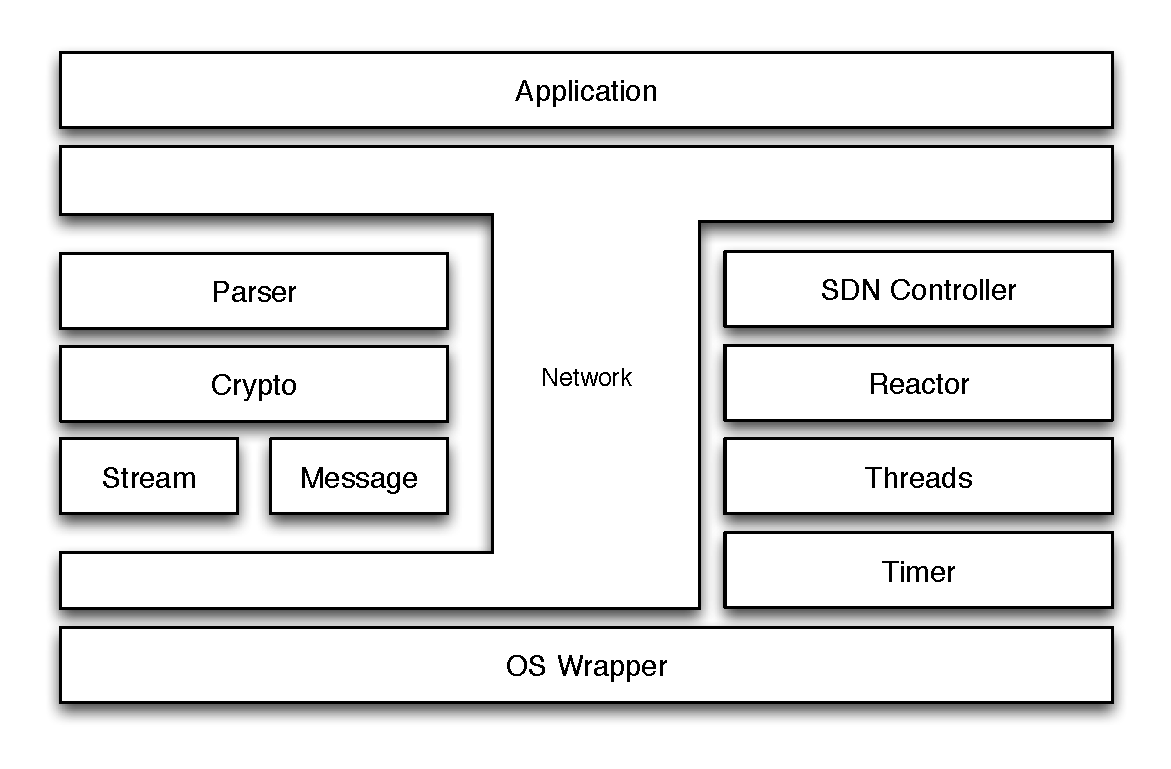
\includegraphics[width=\columnwidth]{Architecture_overview.eps}
\caption{Architecture overview -- this diagram shows that the parser, crypto,
stream and message blocks are separate building blocks which are
interchangeable or omitable.}
\label{fig:arch-overview}
\end{figure}

\section{Methodology}
\begin{thm}[Theorem name]
For a named theorem or theorem-like environment you need to insert
the name through \textsf{Insert\lyxarrow{}Short Title}, as done here.\end{thm}
\begin{lem}
If you don't want a theorem or lemma name don't add one.\end{lem}
\begin{IEEEproof}
And here's the proof!
\end{IEEEproof}

\section{Results}

\begin{figure}[htbp]
\begin{centering}
\textsf{A single column figure goes here}
\par\end{centering}

\caption{Captions go \emph{under} the figure}
\end{figure}
\begin{table}[htbp]
\caption{Table captions go \emph{above} the table}


\centering{}%
\begin{tabular}{|c|c|}
\hline 
delete & this\tabularnewline
\hline 
\hline 
example & table\tabularnewline
\hline 
\end{tabular}
\end{table}



\section{Conclusions}

bla bla


\appendices{}


\section{First appendix}

Citation: \cite{IEEEexample:beebe_archive}


\section{Second appendix}


\section*{Acknowlegment}

bla bla

\bibliographystyle{IEEEtran}
\bibliography{IEEEabrv,IEEEexample,literature}

\begin{IEEEbiography}[{\includegraphics[clip,width=1in,height=1.25in,keepaspectratio,bb = 0 0 200 100, draft, type=eps]{../examples/CV-image.png}}]
{Your Name} All about you and the what your interests are.

\end{IEEEbiography}

\begin{IEEEbiographynophoto}
{Coauthor}Same again for the co-author, but without photo\end{IEEEbiographynophoto}

\end{document}
